\section{Evaluation}\label{sec:eval}

In this section we show the evaluation of our approach. To this end, we
developed several scenarios for WSNs and compare nesC implementations against
its ConesC-written analogs. In addition to the main motivating example described
in Sec.~\ref{sec:appdesign}, we describe two more applications for WSNs.

\subsection{Scenarios}\label{sec:scenarios}

The diagram on Fig.~\ref{fig:shd} displays the possible application of a
Smart-Home scenario, where each room is supplied with one node. The latter
detects a \emph{Light Intensity} and \emph{Climate} by using corresponding
sensors. The node uses actuators to adjusts the luminosity and climate according
to thresholds given by current \emph{Preferences}. The latter depends on the
time of the day and on the day of the week. On the other hand, the system
provides safety by exploiting camera, accelerometer, fire and smoke sensors.
Should the node detects a significant movement, it enables GPRS and sends alert
messages with camera images to the Police. In case of \emph{Fire}, the node
calls the Fire service and communicates with other nodes to allow a householder
to leave the house safely.

\putfigure{caption=Smart-home diagram.,label=fig:shd}{
 \centering
 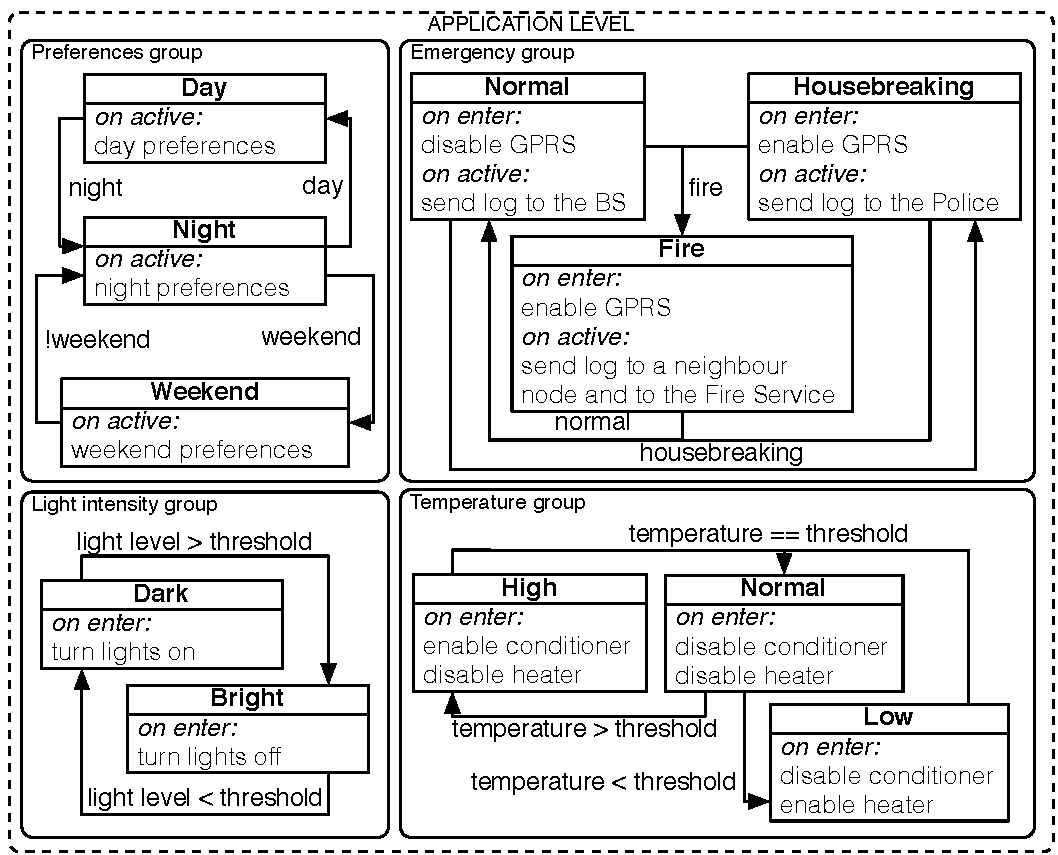
\includegraphics[width=\columnwidth]{pdf/smarthome}
}

Another scenario - a system-level adaptation - is shown on Fig.~\ref{fig:sld}.
If the network is static, it is feasible to use a \emph{Collection Tree
Protocol}. In mobile network, however, a \emph{Gossip}-based protocol shows
better results. Orthogonally to the \emph{Protocol type}, developer may want to
adjust the \emph{Protocol parameters} to enhance a link quality between nodes,
increase the lifetime of the network or use the bandwidth more effectively.

\putfigure{caption=Smart-home diagram.,label=fig:sld}{
 \centering
 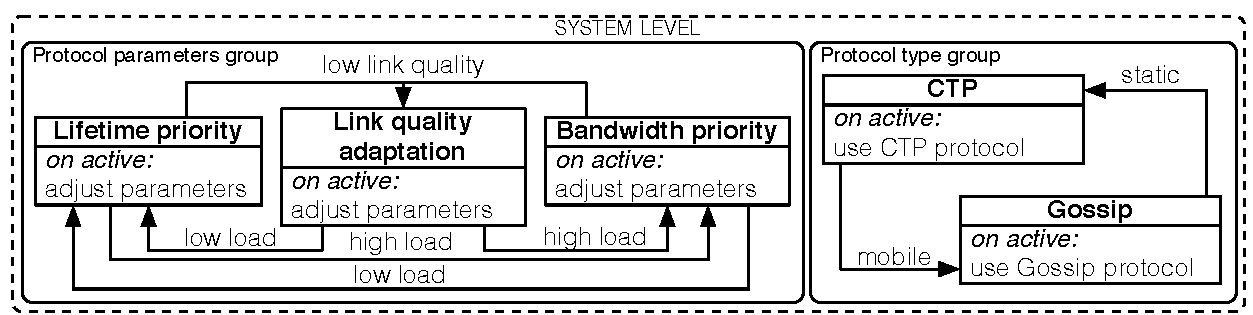
\includegraphics[width=\columnwidth]{pdf/system-level}
}

\subsection{Coupling}\label{sec:evalcomp}

According to the work of Stevens et al.~\cite{stevens79}, there are seven types
of coupling, which are summarized in Table~\ref{tab:couptypes}. It is generally
known that the tightest coupling is, the more difficult is debugging,
maintaining and reusing the program. Coupling types, which are presented in this section, are not forbidden in ConesC, but some of them can be easily avoided with a proper use of its concepts. The result of our analysis, which is displayed on Table~\ref{tab:coupres}, shows that ConesC
implementation is much more decoupled as compared to its nesC counterpart. 

Both implementations have~\emph{External} and~\emph{Data} couplings, since the application is processing the same data differently depending on the current state -- i.e. context in terms of ConesC -- and typed interfaces are used to share the data among modules. We did not use, however, neither messages to share data nor different parts of the same data format, so~\emph{Stamp} and~\emph{Message} couplings are avoided in both implementations.

Implementation of context components in ConesC, example of which are presented in Fig.~\ref{fig:cc} and~\ref{fig:irc}, do not rely on internal work of each other, so the are not coupled in the sense of~\emph{Content coupling}, as compared to nesC-written application, where all the behavioral variations are encapsulated in one module or function. Since each context represents a separate state of the environment or the device the system operates in, contexts are not intended to share any global states, to control the flow of each other and to pass the information how to execute. Our abstraction toward~\emph{context
groups} allows developers to perform system-level operations -- e.g. data storage --
orthogonally to the data processing without actual coupling modules involved.

\begin{table}[!h]
\renewcommand{\arraystretch}{1.3}
\caption{Coupling types.}
\label{tab:couptypes}
\centering
\begin{tabular}{|l|p{2.5in}|}
\hline
\bfseries Type & \bfseries Description\\
\hline
Content (tightest) & One module relies on the internal working of another. Chang- ing one module requires changes in the other as well.\\
\hline
Common & Two or more modules share some global state, e.g., a variable.\\
\hline
External & Two or more modules share a common data format.\\
\hline
Control & One module controls the flow of another, e.g., passing infor- mation that determine how to execute.\\
\hline
Stamp & Two or more modules share a common data format, but each of them uses a different part with no overlapping.\\
\hline
Data & Two or more modules share data through a typed interface, e.g., a function call.\\
\hline
Message (loosest) & Two or more modules share data through an untyped inter- face, e.g., via message passing.\\
\hline
\end{tabular}
\end{table}

\begin{table}[!h]
\renewcommand{\arraystretch}{1.3}
\caption{Coupling comparison.}
\label{tab:coupres}
\centering
\begin{tabular}{|l|l|l|l|l|l|l|l|}
\hline
\bfseries Application & \rotatebox{90}{\bfseries Content} & \rotatebox{90}{\bfseries Common} 
& \rotatebox{90}{\bfseries External} & \rotatebox{90}{\bfseries Control}
& \rotatebox{90}{\bfseries Stamp} & \rotatebox{90}{\bfseries Data}
& \rotatebox{90}{\bfseries Message}\\
\hline
\hline
Wildlife tracking -- nesC &
yes&yes&yes&yes&--&yes&--\\
\hline
Wildlife tracking -- ConesC &
--&--&yes&--&--&yes&--\\
\hline
\hline
Smart-home -- nesC &
yes&yes&yes&yes&--&yes&--\\
\hline
Smart-home -- ConesC &
--&--&yes&--&--&yes&--\\
\hline
\end{tabular}
\end{table}

\subsection{Complexity} 

We estimate the complexity of the program by making use of such indicators as the number of
lines of code (LOC), the number of variable declaration and the number of
functions~\cite{pressman01}. Our results are illustrated on
Table~\ref{tab:compres}. Despite the overall increase of complexity of the whole
application, there is a significant reduction of the per-module complexity.
Context-oriented approach makes a program logically
fragmented, which leads to increased number of modules -- e.g.~\emph{contexts}
and~\emph{context configurations} -- and boilerplate code. Because of the same
reason, functions have to be spitted into smaller isolated parts. We believe, however,
that in larger applications the number of the similar lines of code will be bigger.
The number of LOC can also be decreased significantly -- as showed in Table~\ref{fig:compres} in
parentheses -- by having a tool, which generates a boilerplate code using a diagram of a
context-oriented model of the application, similar to the one displayed in Fig.~\ref{fig:wtd}.
The isolation leads to a code simplification, improved
readability and re-useability along with easier debugging process.

\begin{table}[!h]
\renewcommand{\arraystretch}{1.3}
\caption{Complexity comparison.}
\label{tab:compres}
\centering
\begin{tabular}{|l|c|c|c|c|c|c|}
\hline
&&&& \multicolumn{3}{@{\hspace{0.3em}}c@{\hspace{0.3em}}|}
{\bfseries Average per-module}\\[0.1in]
\bfseries Application & \rotatebox{90}{\bfseries LOC} 
& \rotatebox{90}{\pbox{0in}{\bfseries Variable\\declarations}} 
& \rotatebox{90}{\bfseries Functions} & \rotatebox{90}{\bfseries LOC}
& \rotatebox{90}{\pbox{0in}{\bfseries Variable\\declarations}}
& \rotatebox{90}{\bfseries Functions}\\
\hline
\hline
Wildlife tracking -- nesC&456&17&19&48&6&8\\
\hline
Wildlife tracking -- ConesC&539(440)&17&30&26,5&3&2\\
\hline
Wildlife tracking -- generated&1628&--&--&--&--&--\\
\hline
\hline
Smart-home -- nesC&360&24&28&28&2&2\\
\hline
Smart-home -- ConesC&382(289)&24&56&13&0,8&1,9\\
\hline
Smart-home -- generated&1310&--&--&--&--&--\\
\hline
\hline
Adaptive protocol -- nesC&150&10&13&38&2,5&3,25\\
\hline
Adaptive protocol -- ConesC&191(147)&5&21&14,7&0,4&1,6\\
\hline
Adaptive protocol -- generated&636&--&--&--&--&--\\
\hline
\end{tabular}
\end{table}

\subsection{CPU and memory overhead}

Here we discuss a CPU overhead for context transitions and calls of layered
functions, as well as memory overhead of using ConesC as compared to nesC. To perform a CPU
overhead comparison we use MSPSim emulator~\cite{eriksson09}, while memory overhead was
simply estimated by a nesC compiler at the binary generation.

Since there are neither contexts nor layered functions in nesC-based
implementation, we measured a number of CPU-cycles of parts with different
execution flow. For example, contextual events, like a base station presence,
are detected and handled in ConesC differently as compared to nesC, but,
eventually, it results in the same functionality. Our evaluation shows that CPU overhead of
a layered function call is from 1 to 2 -- depending on the activated context -- CPU-cycles
for~\emph{Battery},~\emph{Base Station} and~\emph{Communication} groups, and from
1 to 3 CPU-cycles for~\emph{Locator} group, which leads us to the linear dependency on the
number of contexts per group. The overhead of context transitions is slightly bigger, but still has
linear dependency on the number of contexts per group: 15 CPU-cycles
for~\emph{Battery},~\emph{Base Station} and~\emph{Communication} groups, and 20
CPU-cycles for~\emph{Locator} group in the worst case. The CPU-overhead of using ConesC is
negligible in terms of energy consumption, since it is even lesser than the simplest operation in
TinyOS -- turning on/off LEDs -- consumes 8 CPU-cycles.

As concerns memory, we have 3\% overhead for Wildlife tracking and 2\% overhead
for Smart-home for both RAM and binary sizes.
